\documentclass[../../main.tex]{subfiles}

\begin{document}

	% Zum iterativen Aufbau des Inklusionsdiagramms. Parameter: 1 -> nur N/N_0; 2 -> bis Z; 3 -> bis Q; 4 -> bis R
	\newcommand{\inclusionDiagram}[1]{
		\begin{tikzpicture}[draw = blue!50!green, font = \small, scale = 0.8]
			\ifnum#1=4
				\draw[fill = blue!50!green!20] (0, 2.75) ellipse (1.8 and 3.75);
				\node[left] at (0, 5.8) {\Real};
				\foreach \i/\j in {(-0.9, 5.2)/\sqrt{2}, (0.7, 5.5)/\pi, (1.1, 4.75)/\sqrt{3}} {
					\node[font = \tiny] at \i {$\j$};
				}
			\fi	
			\ifnum#1>2		
				\draw[fill = blue!50!green!40] (0,2) ellipse (1.6 and 3);
				\node[left] at (0,4) {\Rational};
				\foreach \i/\j in {(-0.9, 3.5)/\frac{2}{3}, (0.25, 4.25)/\frac{1}{2}, (1.1, 3.2)/\frac{7}{8}} {
					\node[font = \tiny] at \i {$\j$};
				}
			\fi
			\ifnum#1>1			
				\draw[fill = blue!50!green!60] (0,1.2) ellipse (1.4 and 2.2);
				\node[left] at (0, 2.6) {\Integer};
				\foreach \i/\j in {(0,3)/-1, (-1, 2)/-2, (1, 1.75)/-3, (0.5,2.3)/-4} {
					\node[font = \tiny] at \i {$\j$};
				}
			\fi
			\ifnum#1>0			
				\draw[fill = blue!50!green!80] (0,0.5) ellipse (1.2 and 1.5);
				\node[left] at (0,1.4) {$\Natural_0$};
				\node[font = \tiny] at (0.5,1.25) {$0$};			
				\draw[fill = blue!50!green] (0,0) circle[radius = 1];
				\node[left] at (0,0) {\Natural};			
				\foreach \i/\j in {(0.5,0.5)/1, (-0.75,-0.25)/2, (0.25,-0.25)/3, (-0.25,-0.75)/4, (-0.3,0.6)/5, (0.75,0)/6} {
					\node[font = \tiny] at \i {$\j$};
				}
			\fi
		\end{tikzpicture}	
	}

	\label{chapter:zahlenmengen}
	\picchangemode
	Wir nutzen Mengen nicht nur, um einfache Alltagsobjekte in Kategorien zu ordnen, wir können auch Mengen verschiedener Zahlen betrachten. Eine besondere Rolle nehmen dabei die Mengen der verschiedenen Zahlentypen ein. Wir wollen diese nun beschreiben, ihnen einen Namen geben und auch ein Symbol zuordnen, durch das wir immer wissen, welche Zahlen gemeint sind.
	
	\parpic{
		\inclusionDiagram{1}
	}
	Als ersten Zahlentyp gibt es die Zahlen, die wir im Alltag zum Zählen verwenden. Das sind die Zahlen $1$, $2$, $3$ und so weiter. Zusammengenommen ergeben sie die Menge der \textbf{natürlichen Zahlen}, für die wir auch einfach \Natural schreiben. Wenn man die Eier in seinem Kühlschrank zählen möchte, verwendet man also genau die natürlichen Zahlen (ein Ei, zwei Eier, drei Eier,$\ldots$). Eine gesonderte Rolle kommt der Zahl $0$ zu. Wir zählen die $0$ nicht als natürliche Zahl (es gibt kein nulltes Ei). Möchte man dennoch zusätzlich die $0$ beim Zählen betrachten (ich habe sechs Eier in meinem Kühlschrank und lege kein weiteres dazu), so schreibt man stattdessen $\Natural_0$. Diese Menge beinhaltet also die Zahlen $0$, $1$, $2$, $3$, $\ldots$ Es gibt allerdings keinen allgemeinen Konsens, ob die $0$ in den natürlichen Zahlen liegt, oder nicht.
	
	Wir wollen aber nicht immer nur aufzählen, also addieren, sondern auch Zahlen voneinander abziehen. Innerhalb der natürlichen Zahlen geht die Subtraktion so lange gut, bis wir eine größere von einer kleineren Zahl abziehen wollen. Zum Beispiel ist $3-7=-4$, was negativ und somit keine natürliche Zahl mehr ist. 
	
	\parpic{
		\inclusionDiagram{2}
	}
	Die natürlichen Zahlen mit $0$ sind eine Teilmenge der sogenannten \textbf{ganzen Zahlen}. Diese verwenden wir, wenn wir nicht nur Objekte aufzählen, sondern von ihrer Anzahl auch wieder etwas abziehen wollen. Den sechs Eiern in meinem Kühlschrank füge ich nach dem Einkauf drei hinzu und verwende fünf, um mir ein Omelett zu machen. Anschließend verbleiben mir vier Eier. Für ein zweites Omelett fehlt mir nun leider ein Ei, da $4-5=-1$ ist. Ganze Zahlen sind also zum einen die natürlichen Zahlen mit $0$, als auch die negativen natürlichen Zahlen $-1$, $-2$, $-3$ und so weiter. Für die Menge der ganzen Zahlen schreiben wir \Integer.
	
	Die zum Abzählen verwendeten Zahlen sind die natürlichen Zahlen. Wir verwenden sie oft, wenn wir im Alltag Dinge addieren wollen. Die ganzen Zahlen erweitern die natürlichen um Subtraktion. Wir können diese Zahlen auch miteinander multiplizieren und erhalten jeweils stets wieder eine natürliche, beziehungsweise ganze Zahl. Neben diesen drei Grundrechenarten hast du in der Schule auch die Division kennengelernt. Auch wie bei der Subtraktion bekommen wir beim Teilen keine Probleme, wenn wir eine Zahl durch einen ihrer Teiler dividieren. So gilt etwa $\frac{8}{4} = 2$, jedoch ist $\frac{2}{5} = 0.4$ keine ganze Zahl mehr.

	\parpic{
		\inclusionDiagram{3}
	}	
	Als nächstes gibt es also die Menge der Bruchzahlen. Diese nennt man \textbf{rationale Zahlen} und schreibt \Rational. Die Menge der rationalen Zahlen besteht also aus allen Zahlen, die wir als Bruch angeben können ($\frac{1}{2}$, $\frac{7}{8}$, $\frac{42}{57}$, $\ldots$). Wir können auch jede ganze Zahl als Bruch angeben, indem wir sie selbst in den Zähler und die $1$ in den Nenner schreiben. So ist zum Beispiel $3 = \frac{3}{1}$. Die Menge der rationalen Zahlen enthält also die Menge der ganzen Zahlen und damit insbesondere auch alle natürlichen Zahlen. Umgekehrt ist zum Beispiel $\frac{1}{2}$ keine ganze Zahl. Insgesamt bilden diese Zahlenmengen eine Kette von echten Teilmengen, wie im Bild dargestellt. Formal können wir hierfür auch mathematische Notationen verwenden und schreiben:
	
	$$\Natural \subsetneq \Natural_0 \subsetneq \Integer \subsetneq \Rational$$
	
	Diese Benennung dieser speziellen Mengen hilft es uns, andere Mengen von Zahlen elegant aufschreiben zu können. Anstatt solche Mengen explizit aufzuzählen oder umständlich zu beschreiben, können wir nun einfach auf unsere Zahlenmengen zurückgreifen.

	\begin{example}{Gerade und ungerade Zahlen}
		Gesucht ist die Menge der geraden Zahlen. Das sind diejenigen ganzen Zahlen, die durch $2$ teilbar sind. Nutzen wir unsere Klassifikation aus, so erhalten wir folgende Definition.
		
		$$\textsc{Gerade} = \left\{x\in\Integer \mid x \text{ ist durch $2$ teilbar}\right\}$$
		
		Auf die selbe Weise können wir auch die Menge der ungeraden Zahlen angeben.
		
		$$\textsc{Ungerade} = \left\{x\in\Integer \mid x \text{ ist nicht durch $2$ teilbar}\right\}$$
	\end{example}
	
	Wir fassen zusammen.
	
	\begin{definition}{Zahlenmengen}
		Wir nennen
		\begin{itemize}
			\item $\Natural = \left\{1,\ 2,\ 3,\ldots \right\}$ die Menge der \textbf{natürlichen Zahlen}
			\item $\Natural_0 = \left\{0, \ 1,\ 2,\ 3,\ldots \right\}$ die Menge der natürlichen Zahlen mit $0$
			\item $\Integer = \left\{\ldots, \ -3, \ -2, \ -1, \ 0, \ 1, \ 2, \ 3, \ldots \right\}$ die Menge der \textbf{ganzen Zahlen}
			\item $\Rational = \left\{ \frac{a}{b} \mid a, \ b \in \Integer \text{ und } b \neq 0\right\}$ die Menge der \textbf{rationalen Zahlen}.
		\end{itemize}
	\end{definition}

	\subsection{Die reellen Zahlen}
	Wir haben jetzt diejenigen Zahlen klassifiziert, mit denen wir im Alltag am meisten zu tun haben. Diese Zahlen können wir nun ihrem Wert entsprechend auf einem Strahl markieren. Einen solchen Strahl nennt man auch Zahlenstrahl. Jeder noch so kleine Punkt auf diesem Strahl (markiert oder nicht) entspricht einer Zahl.
	
	\begin{figure}[h]
		\centering
		\begin{tikzpicture}[scale=5]
			\foreach \x in {-1,0,1} {	
				\draw (\x,8pt)--(\x,-8pt) node[below] {$\x$};	
			}
			\draw (1/2,4pt)--(1/2,-4pt) node[below] {$\frac{1}{2}$};
			\draw (-1/2,4pt)--(-1/2,-4pt) node[below] {$-\frac{1}{2}$};		
			\foreach \x in {1,3}{
				\draw (\x/4,2pt)--(\x/4,-2pt) node[below] {$\frac{\x}{4}$};
				\draw (-\x/4,2pt)--(-\x/4,-2pt) node[below] {$-\frac{\x}{4}$};
			}	
			\foreach \x in {1,3,5,7}{
				\draw (\x/8,1pt)--(\x/8,-1pt) node[below] {$\frac{\x}{8}$};
				\draw (-\x/8,1pt)--(-\x/8,-1pt) node[below] {$-\frac{\x}{8}$};
			}
			\draw (-1.1,0)--(1.1,0);
		\end{tikzpicture}
		\caption{Ein Ausschnitt eines beispielhaften Zahlenstrahls. Eingezeichnet sind die ganzen Zahlen $-1,\ 0$ und $1$ sowie ein paar ausgewählte (aber nicht alle) Bruchzahlen, die dazwischen liegen. Der Strahl kann auf beiden Seiten weiter fortgeführt werden.}
	\end{figure}

	 Aus Platzgründen können wir natürlich nicht jede Zahl markieren, wir treffen stattdessen eine Auswahl. Im obigen Bild haben wir etwa auf die Markierung von $\frac{1}{3}$ verzichtet. Dieser Wert liegt in der Lücke zwischen $\frac{1}{4}$ und $\frac{3}{8}$. Man kann sich nun die Frage stellen, ob wir mit den rationalen Zahlen auf so einem Zahlenstrahl jeden möglichen Punkt markieren können. Wenn wir also jede einzelne rationale Zahl, die es gibt, auf einem Zahlenstrahl markieren, gibt es dann Punkte auf dem Strahl, die wir nicht markiert haben? Anders gefragt, gibt es vielleicht Zahlen, die \textbf{nicht} rational sind, die man also nicht als Bruch darstellen kann? 

	Vielleicht ist dir aufgefallen, dass die Mengen \Natural, \Integer und \Rational in einem gewissen Zusammenhang zu unseren Grundrechenarten stehen. Die natürlichen Zahlen mit Zählen, also Addition, die ganzen Zahlen zusätzlich mit Subtraktion und die rationalen Zahlen mit Division (natürlich können wir diese Zahlen auch immer zur Multiplikation verwenden). Im Kapitel (ref?) hast du zusätzlich Wurzeln kennengelernt. Wir wollen uns nun überlegen, ob die Wurzeln positiver rationaler Zahlen noch allesamt in \Rational liegen.	
	
	In manchen Fällen ist die Sache klar. Zum Beispiel ist $\sqrt{9}=3$ eine natürliche Zahl und liegt somit in \Rational. Andere Wurzeln sind leider nicht so eindeutig, wie etwa $\sqrt{2}$. Der Wert von $\sqrt{2}$ liegt irgendwo zwischen $1$ und $2$ und ist damit nicht mehr natürlich. Tatsächlich ist er aber auch nicht rational, wie das folgende Resultat zeigt.
	
	\begin{theorem}{Nicht alle Zahlen sind rational}
		Es gibt Zahlen, die nicht rational sind. Man kann also nicht jede Zahl als Bruchzahl darstellen. Im Speziellen ist etwa $\sqrt{2} \notin\Rational$.
	\end{theorem}
	
	\begin{proof}
		Wir zeigen, dass $\sqrt{2}$ nicht rational ist durch einen Widerspruchsbeweis. Ist $\sqrt{2}$ eine rationale Zahl, so können wir sie als Bruch aufschreiben. Das heißt, es gibt ganze Zahlen $a, \ b\in\Integer$ mit $b \neq 0$, sodass gilt
		
		$$\sqrt{2} = \frac{a}{b}.$$
		
		Wir nehmen hierbei an, dass es sich bei $\frac{a}{b}$ bereits um einen gekürzten Bruch handelt (andernfalls kürzen wir so lange, bis wir einen gekürzten Bruch erhalten). Das bedeutet, dass die Zahlen $a$ und $b$ keinen gemeinsamen Teiler mehr besitzen. Wenn wir obige Gleichung auf beiden Seiten quadrieren, erhalten wir
		
		$$2 = \frac{a^2}{b^2}.$$
		
		Multiplikation mit $b^2$ auf beiden Seiten liefert dann
		
		$$2b^2 = a^2.$$ 
		
		Also ist $a^2$ eine gerade Zahl. Daraus folgt, dass auch $a$ gerade sein muss. Wir können $a$ also schreiben als 
		$a = 2k$, wobei $k$ eine ganze Zahl ist. Setzen wir dies oben für $a$ ein, erhalten wir
		
		$$2b^2 = \left(2k\right)^2 = 4k^2.$$
		
		Division mit $2$ auf beiden Seiten liefert dann
		
		$$b^2 = 2k^2$$
		
		und folglich ist $b^2$, und damit insbesondere auch $b$ selber gerade. Wir haben jetzt gezeigt, dass sowohl $a$, als auch $b$ gerade Zahlen sind. Damit können wir den Bruch $\frac{a}{b}$ aber weiter kürzen, was ein Widerspruch zu unserer Annahme darstellt. Daher kann $\sqrt{2}$ nicht als Bruch dargestellt werden.
	\end{proof}

	\parpic{
		\inclusionDiagram{4}
	}
	Tatsächlich sind Wurzeln von Primzahlen niemals rational. Auch andere Zahlen, wie die Kreiszahl $\pi$ sind nicht in \Rational enthalten. Auf unserem Zahlenstrahl liegen diese Zahlen in den Lücken zwischen rationalen Zahlen. Die Menge, die alle Zahlen des Zahlenstrahls enthält, nennen wir die Menge der \textbf{reellen Zahlen} \Real, die wir an dieser Stelle nicht formal definieren wollen. Jeder beliebige Punkt auf dem Zahlenstrahl ist somit eine reelle Zahl.
	
	Die reellen Zahlen enthalten also die rationalen Zahlen. Wie wir gesehen haben, gibt es aber auch reelle Zahlen, die nicht rational sind (zum Beispiel $\sqrt{2}$). Diese Zahlen nennt man dann \textbf{irrational}. Dementsprechend können wir die Kette unserer Zahlenmengen wie folgt um die reellen Zahlen erweitern. 
	
	$$\Natural \subsetneq \Natural_0 \subsetneq \Integer \subsetneq \Rational \subsetneq \Real$$
		
	\begin{nutshell}{Zahlenmengen}
		Alle Zahlen, denen wir im Alltag begegnen, können wir mithilfe von Mengen klassifizieren.
		\begin{itemize}
			\item $\Natural = \left\{1,\ 2,\ 3,\ldots \right\}$ die Menge der \textbf{natürlichen Zahlen}
			\item $\Natural_0 = \left\{0, \ 1,\ 2,\ 3,\ldots \right\}$ die Menge der natürlichen Zahlen mit $0$
			\item $\Integer = \left\{\ldots, \ -3, \ -2, \ -1, \ 0, \ 1, \ 2, \ 3, \ldots \right\}$ die Menge der \textbf{ganzen Zahlen}
			\item $\Rational = \left\{ \frac{a}{b} \mid a, \ b \in \Integer \text{ und } b \neq 0\right\}$ die Menge der \textbf{rationalen Zahlen}
			\item \Real die Menge der \textbf{reellen Zahlen}, die aus allen Zahlen auf dem Zahlenstrahl besteht.
		\end{itemize}
		Diese Mengen bilden eine Kette strikter Teilmengen. Diese Teilmengenbeziehung lässt sich am unteren Mengendiagramm ablesen.
		\begin{center}
			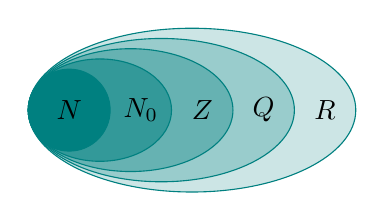
\begin{tikzpicture}[scale=1.3, draw = blue!50!green]
				\draw[fill = blue!50!green!20]  (1.2,0) ellipse (1.6 and 0.8);
				\node at (2.5,0) {$\mathbb{R}$};
				\draw[fill = blue!50!green!40]  (0.9,0) ellipse (1.3 and 0.7);
				\node at (1.9,0) {$\mathbb{Q}$};
				\draw[fill = blue!50!green!60]  (0.6,0) ellipse (1 and 0.6);
				\node at (1.3,0) {$\mathbb{Z}$};
				\draw[fill = blue!50!green!80]  (0.3,0) ellipse (0.7 and 0.5);
				\node at (0.7,0) {$\mathbb{N}_0$};
				\draw[fill = blue!50!green] (0,0) circle[radius=0.4];
				\node at (0,0) {$\mathbb{N}$};
			\end{tikzpicture}
		\end{center}
	\end{nutshell}
\nopicchangemode	
\end{document}
